\documentclass[twoside]{article}

\usepackage[math]{kurier}
\usepackage[sc]{mathpazo}   
\renewcommand{\sfdefault}{kurier}

\usepackage[boxruled]{algorithm2e}
\usepackage[utf8]{inputenc}
\usepackage[backend=biber]{biblatex}
\usepackage[english]{babel}
\usepackage[english]{babel}
\usepackage[autostyle]{csquotes}
\usepackage{placeins}
\usepackage[backend=biber]{biblatex}
\bibliography{./lecture_11_biblio_.bib}

\usepackage{graphics}
\usepackage{graphicx}
\usepackage{subcaption}
\usepackage{amsmath}
\usepackage{float}
\setlength{\oddsidemargin}{0.25 in}
\setlength{\evensidemargin}{-0.25 in}
\setlength{\topmargin}{-0.6 in}
\setlength{\textwidth}{6.5 in}
\setlength{\textheight}{8.5 in}
\setlength{\headsep}{0.75 in}
\setlength{\parindent}{0 in}
\setlength{\parskip}{0.1 in}


\newcounter{lecnum}
\renewcommand{\thepage}{\thelecnum-\arabic{page}}
\renewcommand{\thesection}{\thelecnum.\arabic{section}}
\renewcommand{\theequation}{\thelecnum.\arabic{equation}}
\renewcommand{\thefigure}{\thelecnum.\arabic{figure}}
\renewcommand{\thetable}{\thelecnum.\arabic{table}}


\newcommand{\lecture}[4]{
   \pagestyle{myheadings}
   \thispagestyle{plain}
   \newpage
   \setcounter{lecnum}{#1}
   \setcounter{page}{1}
   \noindent
   \begin{center}
   \framebox{
      \vbox{\vspace{2mm}
    \hbox to 6.28in { {\bf \sffamily AA 274: Principles of Robotic Autonomy
                        \hfill Winter 2018} }
       \vspace{4mm}
       \hbox to 6.28in { {\sffamily{\Large \hfill Lecture #1: #2  \hfill}} }
       \vspace{2mm}
       \hbox to 6.28in { {\it \hfill Scribes: #4} }
      \vspace{2mm}}
   }
   \end{center}
   \markboth{Lecture #1: #2}{Lecture #1: #2}

   \vspace*{4mm}
}


%%%%%%%%%%%%%%%%%%%%%%%%%%
%document
\begin{document}
%modify this
\lecture{11}{Localization Filters}{}{Arthur Binstein, Anqi Fu, Trevor Halsted, Scott Hemley, Alexander Hobbs, Jialong Wang}

\section{Introduction}

The first part of this lecture covers filtering techniques including parametric and non-parametric filters. The parametric filters include the Kalman Filter, the Extended Kalman Filter and the Unscented Kalman Filter, while the non-parametric filters covered are the histogram and particle filters. The second part of this lecture is a brief introduction to robot localization.

\section{Parametric Filters}
Parametric filters are a family of state estimators that assume the form of a robot's belief distribution and calculate the parameters to fully define that distribution based on the latest information. In particular, Gaussian filters are an important group of parametric filters that assume the belief distribution is a multivariate normal distribution. The Kalman filter and its variants belong to this group of parametric filters.

%\FloatBarrier
\begin{figure}[b]
\centering
\begin{subfigure}{.5\textwidth}
  \centering
  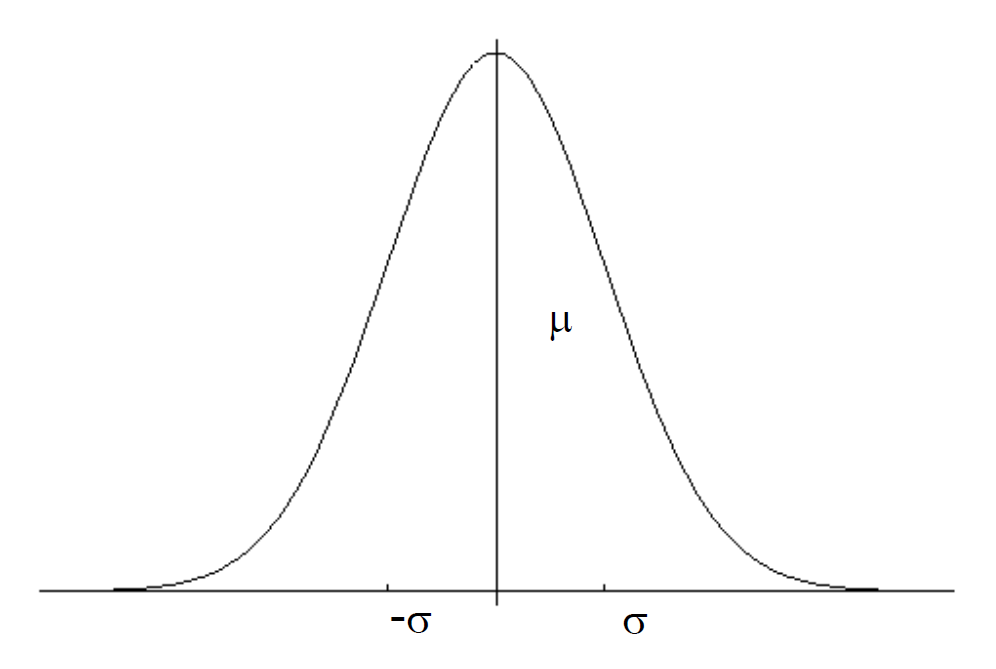
\includegraphics[width=.9\linewidth]{gaussian_univariate.png}
  \caption{Gaussian Distribution in One Variable}
  \label{fig:EKF_best}
\end{subfigure}%
\begin{subfigure}{.5\textwidth}
  \centering
  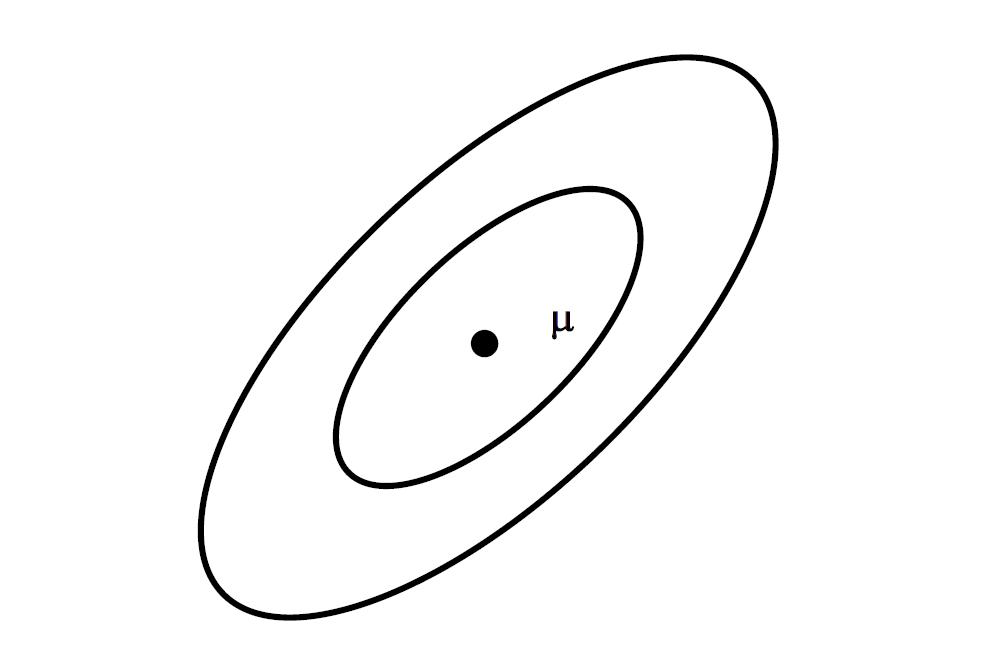
\includegraphics[width=.9\linewidth]{gaussian_multivariate.png}
  \caption{Level Curves of Gaussian Distribution in Two Variables}
  \label{fig:EKF_bad}
\end{subfigure}
\caption{Visualizations of the multivariate normal (Gaussian) distribution \cite{Xmisc}.}
\label{fig:Gaussians}
\end{figure}
%\FloatBarrier

\subsection{Kalman Filter}
\subsubsection{Setup}
A Kalman filter $K_t$ uses a model of the system dynamics, known control inputs to a system, and noisy measurements to estimate the robot's state. The algorithm calculates weights on the state predicted from the measurements and the state predicted by the model. The key idea behind Kalman filters is that we assume that each belief function (the expected state) follows a multivariate normal distribution (Gaussian distribution), illustrated in Figure \ref{fig:Gaussians}. However, instead of propagating the probability density function itself, we choose to propagate forward the project state (mean) and covariance.

\par
In general, the linearity assumption does not hold (e.g., square root in Euclidean distance calculation) when modeling the robot. But we make several assumptions when using Kalman filters that simplify the problem.
First we assume a linear dynamics model of the robot:
\begin{equation}
x_t = A_t x_{t-1} + B_t u_t + \epsilon_{t}
\end{equation}
where $\epsilon_{t}$ is the independent process noise with variance $R_t$. Notice here that the probability generative model now is also Gaussian because the Gaussian of a linear equation is still Gaussian. Second we assume that the measurement model is also linear
\begin{equation}
z_t = C_t x_t + \delta_t
\end{equation}
where $\delta_t$ is the independent measurement noise with variance $Q_t$. This ensures the measurement probability is also a Gaussian. The third and last assumption is that the initial belief function is also Gaussian in the form of \begin{equation}
bel(x_0) = \mathtt{det}(2\pi\Sigma_0)^{-\frac{1}{2}}\mathtt{exp}(-\frac{1}{2}(x_0-\mu_0)\Sigma_0^{-1}(x_0-\mu_0)^{T})
\end{equation} 
such that our posterior $bel$ functions will also follow Gaussian distribution.
\subsubsection{Algorithm}
First we make a prediction of the state and project mean and covariance ahead,
\begin{align}
\begin{split}
\bar{\mu}_t &= A_t\mu_{t-1}+B_t u_t \\
\bar{\Sigma}_t &= A_t\Sigma_{t-1} A_t^{T} + R_t
\end{split}
\label{LinDyn}
\end{align}
Then we need to correct the prediction with our measurement. First we compute the Kalman gain,
\begin{equation}
K_t = \bar{\Sigma}_{t}C_t^{T}(C_t\bar{\Sigma}_{t}C_t^{T}+Q_t)^{-1}
\end{equation}
Then we update our belief function 
\begin{align}
\begin{split}
\mu_t &= \bar{\mu}_t + K_t(z_t-C_t\bar\mu_{t})\\
\Sigma_t &= (I-C_t K_t)\bar{\Sigma}_t
\end{split}
\label{KF}
\end{align}
Repeat this process.
A few iterations of this algorithm are depicted in Figure \ref{fig:KF_algorithm}.

\SetKwInput{KwReturn}{Return}
\begin{algorithm}[H]
\caption{Kalman Filter}
	\KwData{$(\mu_{t-1}, \Sigma_{t-1}), u_t, z_t$}
	\KwResult{$\left(\mu_t, \Sigma_t\right)$}
	$	\bar{\mu}_t = A_t\mu_{t-1}+B_t u_t$\;
	$	\bar{\Sigma}_t = A_t\Sigma_{t-1} A_t^{T} + R_t$\;	
	$ 	K_t = \bar{\Sigma}_{t}C_t^{T}(C_t\bar{\Sigma}_{t}C_t^{T}+Q_t)^{-1}$\;	
	$    \mu_t = \bar{\mu}_t K_t(z_t-C_t\bar\mu_{t})$\;	
	$   \Sigma_t = (I-C_t K_t)\bar{\Sigma}_t$\;
	\KwReturn{$(\mu_t, \Sigma_t)$}
\end{algorithm}

%\FloatBarrier
\begin{figure}[tp]
\centering
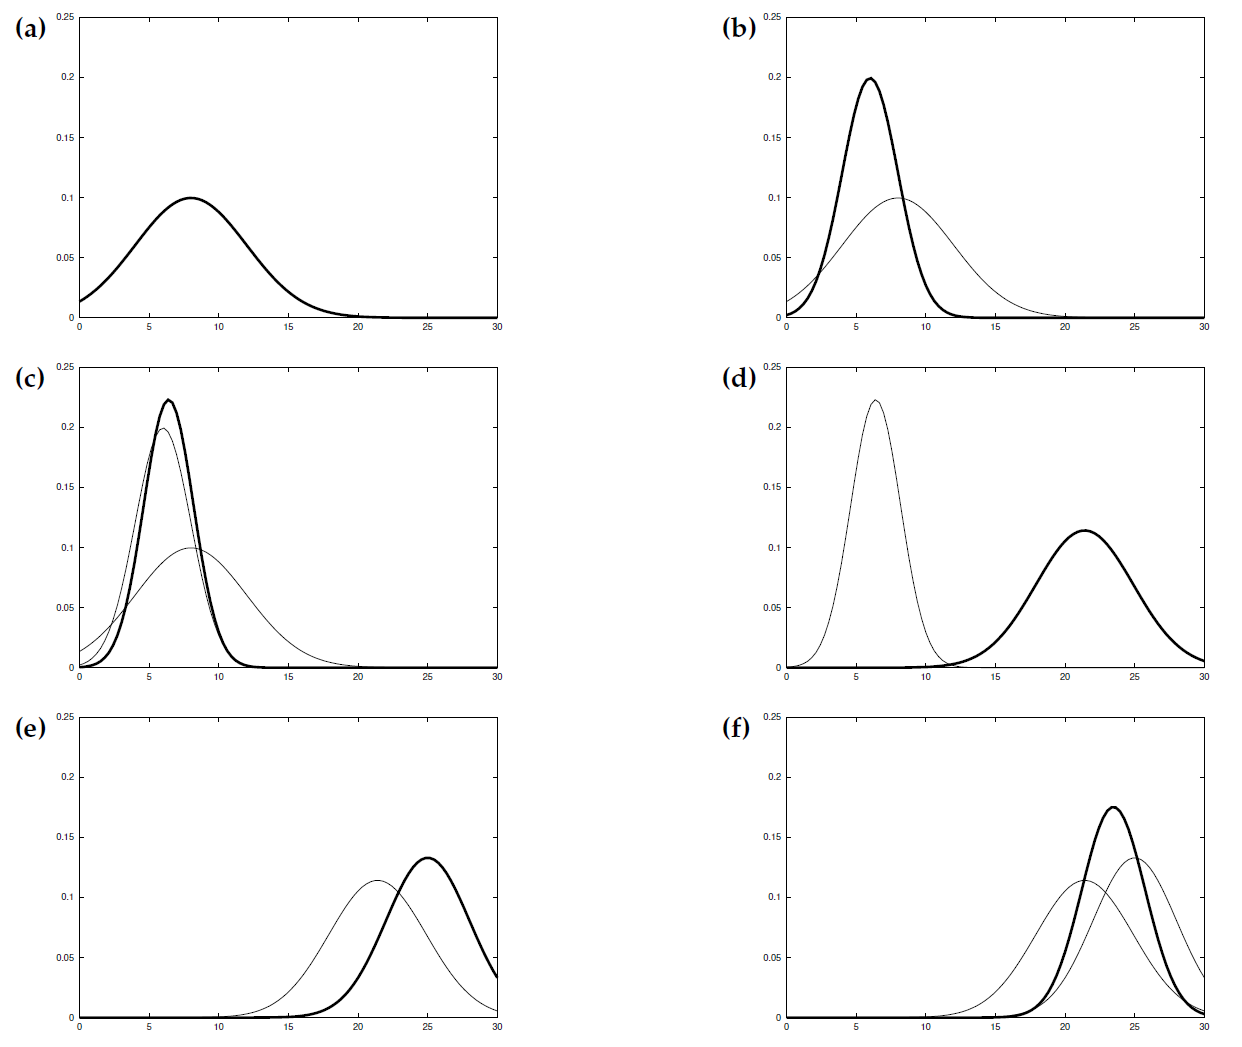
\includegraphics[width=1\linewidth]{KF_algorithm.png}
\caption{Visualization of the Kalman Filter Algorithm from \cite{thrun2005probabilistic}. Current step is in bold and previous data are in gray: (a) the initial belief distribution, (b) the measurement with uncertainty in bold and initial belief in gray, (c) updated belief in bold with previous belief and measurement in gray, (d) belief after motion to the right with added uncertainty in bold and previous belief in gray, (e) new measurement with uncertainty in bold and latest belief in gray, and (f) the updated belief in bold with previous belief and measurement in gray.}
\label{fig:KF_algorithm}
\end{figure}
%\FloatBarrier

\subsubsection{Derivation}
The following recursive update equation can be derived by applying Bayes rule to the posterior distribution:
\begin{equation}
p(x_t \mid z_{1:t}, u_{1:t}) = \eta p(z_t \mid x_t, z_{1:t-1}, u_{1:t})p(x_t \mid z_{1:t-1}, u_{1:t}).
\end{equation} Noting that conditional independence gives the simplification
\begin{equation}
p(x_t \mid z_{1:t}, u_{1:t}) = \eta p(z_t \mid x_t)p(x_t \mid z_{1:t-1}, u_{1:t}). \label{predbel0}
\end{equation}
Given, $\overline{bel}(x_t) = p(x_t \mid z_{1:t-1},u_{1:t})$, we can assume that the state is complete to obtain the recursive update equation:
\begin{equation}
\overline{bel}(x_t) = \int p(x_t \mid x_{t-1}, u_t) p(x_{t-1} \mid z_{1:t-1}u_{1:t-1}) dx_{t-1}
\end{equation}
which can also be expressed as
\begin{equation}
\overline{bel}(x_t) = \int p(x_t \mid x_{t-1}, u_t) bel(x_{t-1}) dx_{t-1} \label{predbel}
\end{equation}
Since $x_t = A_tx_{t-1} + B_tu_t + \epsilon_t$ with $\epsilon_t \sim \mathcal{N}(\mu_t, R_t)$, we know that $p(x_t \mid x_{t-1}, u_t) \sim \mathcal{N}(A_tx_{t-1} + B_tu_t, R_t)$. Similarly, the Linear-Gaussian assumptions described above guarantee that $bel(x_{t-1}) \sim \mathcal{N}(\mu_{t-1}, \Sigma_{t-1}$. Then \eqref{predbel} can be simplified to
\begin{equation}
\overline{bel}(x_t) = \mathcal{N}(\bar{\mu}_t, \bar{\Sigma}_t) \label{predbel2}
\end{equation}
where $\bar{\mu}_t = A_t\mu_{t-1} + B_t u_t$ and $\bar{\Sigma}_t = A_t \Sigma_{t-1} A_t^T + R_t$ from integrating the product of the Gaussian distributions. Thus, the prediction step can be summarized with \eqref{predbel2}.
From \eqref{predbel0}, we have the following relationship between the posterior distribution and the predicted belief:
\begin{equation}
bel(x_t) = \eta p(z_t \mid x_t) \overline{bel}(x_t).
\end{equation}
The assumptions of a linear-Gaussian system provide that $p(z_t \mid x_t) \sim \mathcal{N}(Cx_t, Q_t)$ and that $\overline{bel}(x_t) \sim \mathcal{N}(\bar{\mu}_t, \bar{\Sigma}_t)$. Noting that the product of two Gaussians is Gaussian, we have
\begin{equation}
bel(x_t) = \mathcal{N}(\mu_t, \Sigma_t),
\end{equation}
for which the equations for $\mu_t$, and $\Sigma_t$ can be expressed as in \eqref{KF}.

%%%%%%%%%%%%%%%%%%%%%%%%%%%%%%%%%%%%%%%%%%%%%%%%%%
\subsection{Extended Kalman Filter (EKF)}

The Extended Kalman Filter (EKF) is a Kalman Filter that relaxes the linearity assumption of the models. Instead of trying to find the exact posterior solution, it seeks to compute a Gaussian approximation.  The belief distribution is passed through the filter and results in a non-Gaussian distribution. Then we find the best Gaussian fit to this resulting distribution.
\par
The assumption in EKF is that we can use the first-order Taylor expansion to linearize $g$ and $h$ around the most likely state (e.g. the mean of the state), then pass beliefs through linearized models. For the dynamics equation, we propagate the state as $x_t = g(u_t, x_{t-1})$, with $g(u_t, x_{t-1})$ in the form of
\begin{equation}
	g(u_t, x_{t-1}) \approx g(u_t, \mu_{t-1}) + J_g(u_t, \mu_{t-1})(x_{t-1}-\mu_{t-1})
\end{equation}
where $J_g$ is the Jacobian matrix of the function $g$. Using the notation $G_t = J_g(u_t, \mu_{t-1})$, the probability distribution of the state at time $t$ given the state at time $t-1$ and the control action taken at time $t$ is expressed as
\begin{equation}\footnotesize
p(x_t \mid u_t, x_{t-1}) = \det \left(2\pi R_t\right)^{-1/2} \exp \left(-\frac{1}{2}\left[x_t - g(u_t, \mu_{t-1}) - G_t\cdot (x_{t-1} - \mu_{t-1})\right]^T R_t^{-1} \left[x_t - g(u_t, \mu_{t-1}) - G_t\cdot(x_{t-1} - \mu_{t-1})\right]\right)
\end{equation}
And for the measurement model $z_t = h(x_t)$, where
\begin{equation}
	h(x_t) = h(\bar{\mu}_{t})+J_h(\bar{\mu}_{t})(x_t-\bar{\mu}_{t})
\end{equation}
The Jacobian of the measurement function is $J_h({\bar{\mu}_t})$, for which we use the notation $H_t$. Then the probability distribution of the measurement given the state at time $t$ is
\begin{equation}
p(z_t \mid x_t) = \det(2\pi Q_t)^{-1/2} \exp \left( -\frac{1}{2} \left[z_t - h(\bar{\mu}_t) - H_t \cdot (x_t - \bar{\mu}_t)\right]^T Q_t^{-1}\left[z_t - h(\bar{\mu}_t) - H_t \cdot (x_t - \bar{\mu}_t)\right]\right)
\end{equation}

A comparison of the linearity requirement of the standard Kalman Filter and the performance of the EKF on a nonlinear function that violates this requirement is shown in Figure \ref{fig:KF_vs_EKF}.

%\FloatBarrier
\begin{figure}[tp]
\centering
\begin{subfigure}{.5\textwidth}
  \centering
  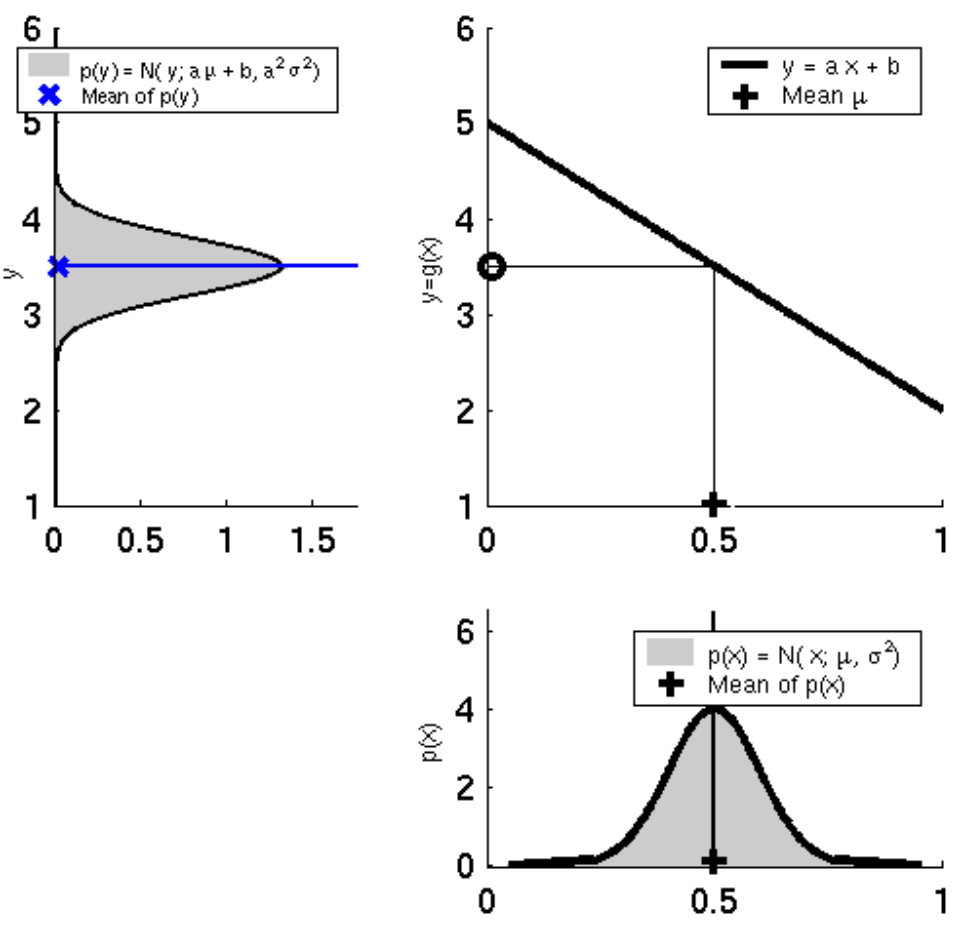
\includegraphics[width=.9\linewidth]{KF_linearity.png}
  \caption{Kalman Filter Linearity Assumption}
  \label{fig:KF_linearity}
\end{subfigure}%
\begin{subfigure}{.5\textwidth}
  \centering
  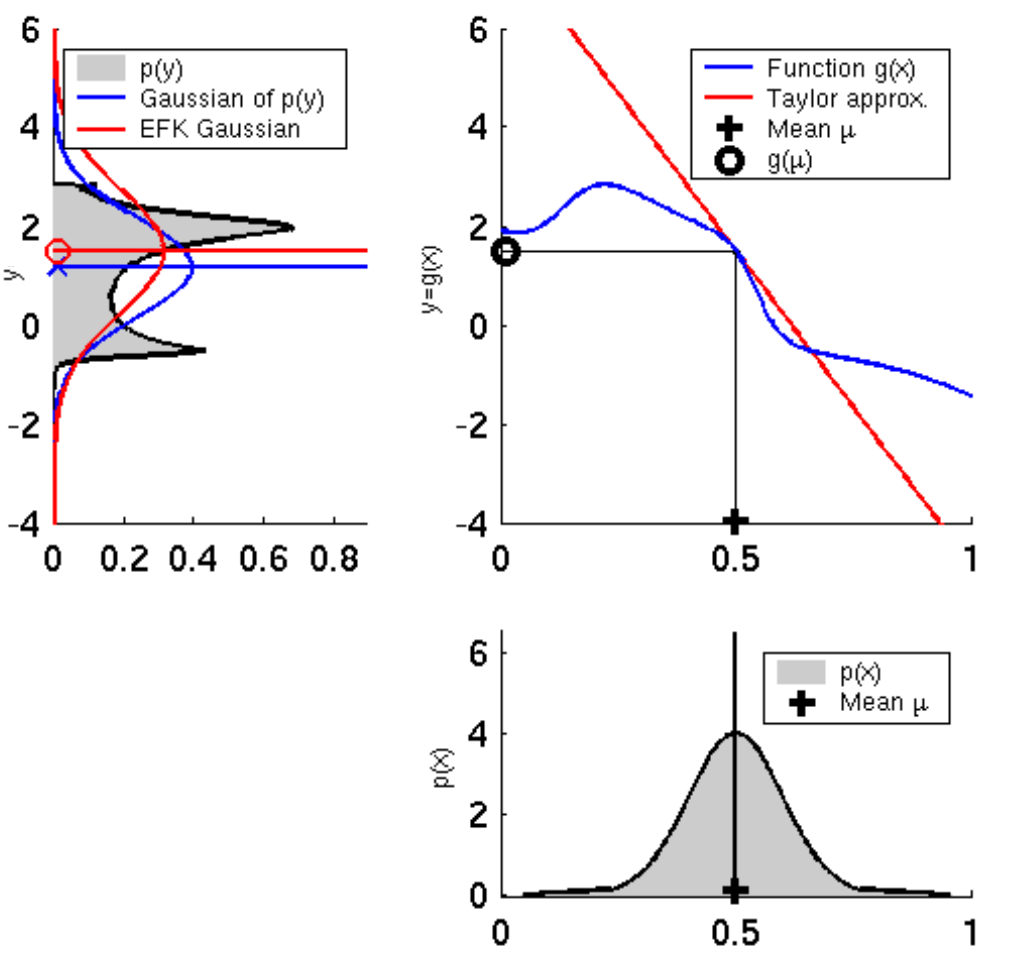
\includegraphics[width=.9\linewidth]{EKF_med_var.png}
  \caption{EKF Linearization}
  \label{fig:EKF_med_var}
\end{subfigure}
\caption{Comparison of (a) the linearity assumption of the standard Kalman Filter \cite{Xmisc} and (b) its extension to nonlinear functions through linearization \cite{Xmisc}.}
\label{fig:KF_vs_EKF}
\end{figure}
%\FloatBarrier

\subsubsection{EKF Algorithm}
Unlike ordinary Kalman Filters, the EKF algorithm uses Jacobian matrices of the linearized model $g$ and $h$ instead of the linear system matrices. 
In the prediction step we propagate forward the expected value of the state assuming no noise. We also replace the covariance matrix $A_t$ with Jacobian $G_t$ from the linearization. While in the correction step we replace $C_t$ in the Kalman gain with Jacobian $H_t$. The linearized dynamics equations in \eqref{LinDyn} are replaced by the following:
\begin{align}
\begin{split}
\bar{\mu}_t &= g(u_t,\mu_{t-1})
\\\bar{\Sigma}_t &= G_t\Sigma_{t-1} G_t^{T} + R_t
\end{split}
\end{align}
Then we need to correct the prediction with our measurement. First we compute the Kalman gain,
\begin{equation}
K_t = \bar{\Sigma}_{t}H_t^{T}(H_t\bar{\Sigma}_{t}H_t^{T}+Q_t)^{-1}
\end{equation}
Then we update our belief function 
\begin{align}
\begin{split}
\mu_t &= \bar{\mu}_t+K_t(z_t-h(\mu_{t})) \\
\Sigma_t &= (I-K_t H_t)\bar{\Sigma}_t
\end{split}
\end{align}
Repeat this process.

\begin{algorithm}[H]
\caption{Extended Kalman Filter}
\KwData{$(\mu_{t-1}, \Sigma_{t-1}), u_t, z_t$}
	\KwResult{$\left(\mu_t, \Sigma_t\right)$}
	$	\bar{\mu}_t = g(u_t,\mu_{t-1})$\;
	$	\bar{\Sigma}_t = G_t\Sigma_{t-1} G_t^{T} + R_t$\;	
	$ 	K_t = \bar{\Sigma}_{t}H_t^{T}(H_t\bar{\Sigma}_{t}H_t^{T}+Q_t)^{-1}$\;	
	$    \mu_t = \bar{\mu}_t+K_t(z_t-h(\mu_{t}))$\;	
	$   \Sigma_t = (I-K_t H_t)\bar{\Sigma}_t$\;
	\KwReturn{$(\mu_t, \Sigma_t)$}
\end{algorithm}

\subsubsection{EKF Results}
The accuracy of the linearity assumption in the EKF is strongly dependent on the variance. Linearizing around the mean is only valid for points that are near the mean. So if the variance is low, as in Figure \ref{fig:EKF_low_var}, the EKF provides an accurate estimate of the true state. If there is high variance in the prior distribution, as in Figure \ref{fig:EKF_high_var}, the EKF will propagate forward a poor estimate of a poor estimate, and can become very ineffective. 

%\FloatBarrier
\begin{figure}[H]
\centering
\begin{subfigure}{.5\textwidth}
  \centering
  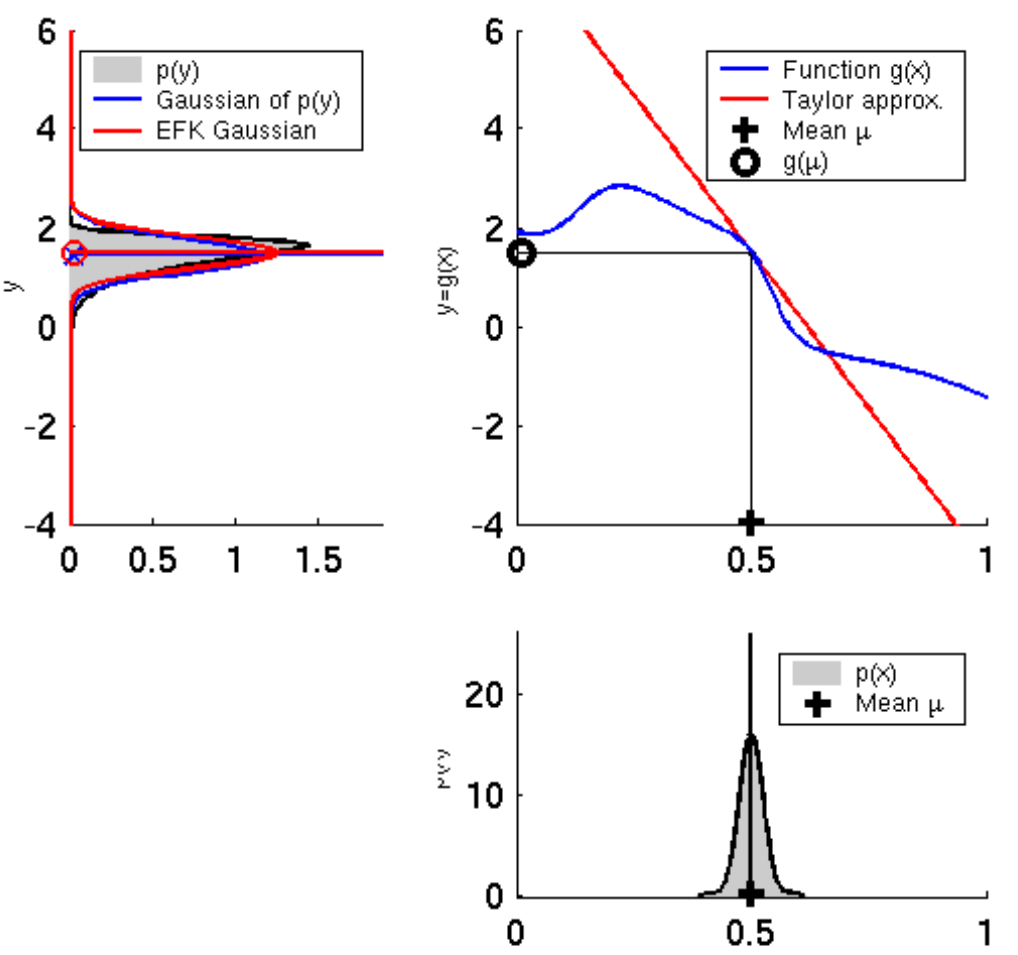
\includegraphics[width=.9\linewidth]{EKF_low_var.png}
  \caption{EKF With Low Variance}
  \label{fig:EKF_low_var}
\end{subfigure}%
\begin{subfigure}{.5\textwidth}
  \centering
  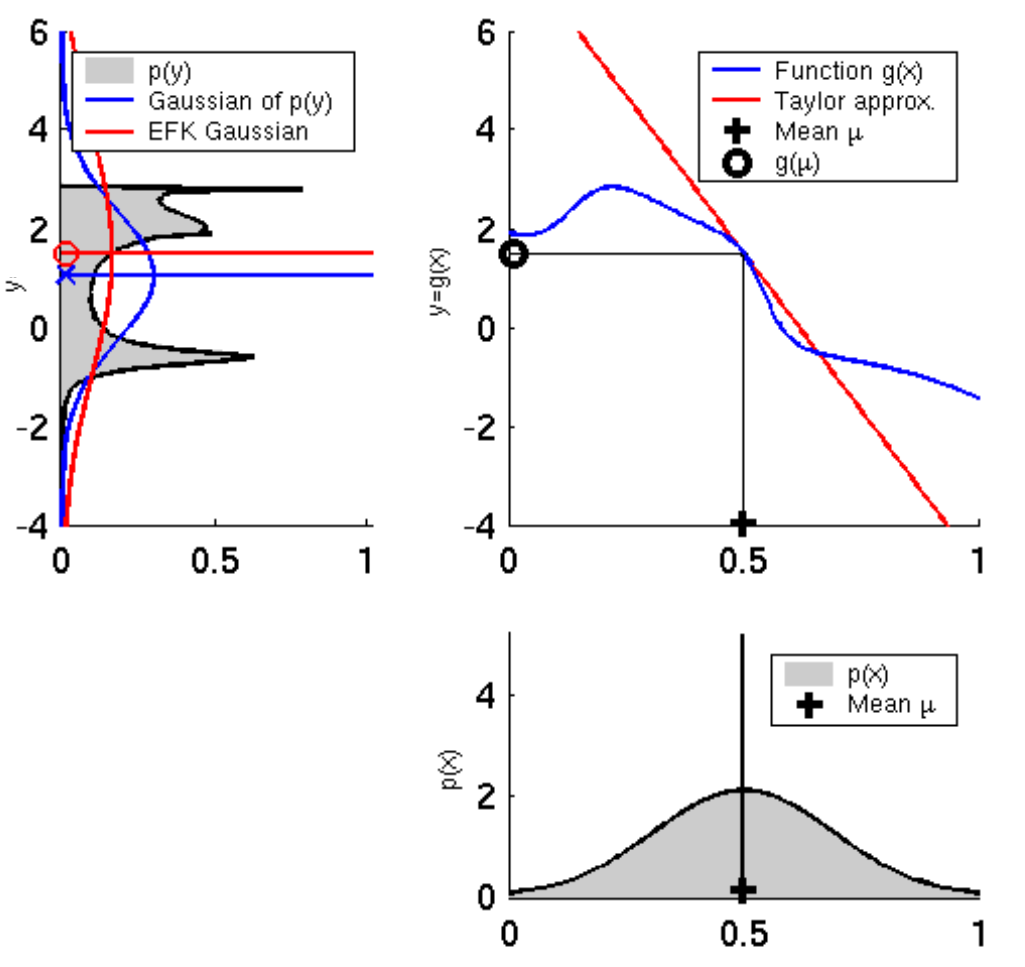
\includegraphics[width=.9\linewidth]{EKF_high_var.png}
  \caption{EKF With High Variance}
  \label{fig:EKF_high_var}
\end{subfigure}
\caption{EKF performance for different levels of uncertainty \cite{Xmisc}.}
\label{fig:EKF_variance}
\end{figure}
%\FloatBarrier


\subsection{Unscented Kalman Filter (UKF)}

Where in EKF, a Gaussian prediction is propagated through a simplified dynamic model, in UKF an approximated belief is propagated through the correct nonlinear model. This is accomplished by choosing points near the mean, called sigma points, transforming these points using the nonlinear model, and computing a posterior Gaussian distribution using these transformed sigma points. The differences between the treatment on nonlinearities in the EKF and UKF are illustrated in Figure \ref{fig:EKF_vs_UKF_transform}.

%\FloatBarrier
\begin{figure}[t]
\centering
\begin{subfigure}{.5\textwidth}
  \centering
  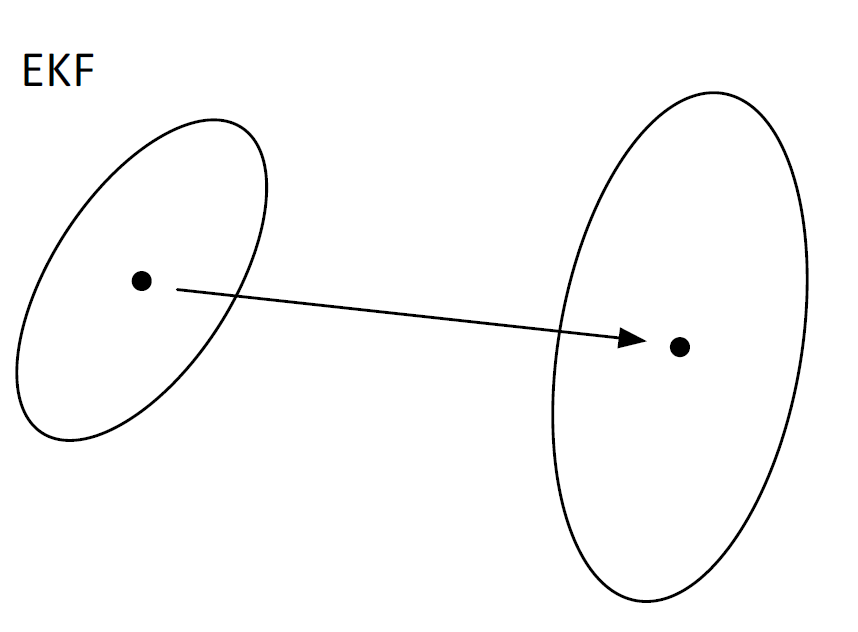
\includegraphics[width=.75\linewidth]{EKF_transform.PNG}
  \caption{EKF Transform}
  \label{fig:EKF_transform}
\end{subfigure}%
\begin{subfigure}{.5\textwidth}
  \centering
  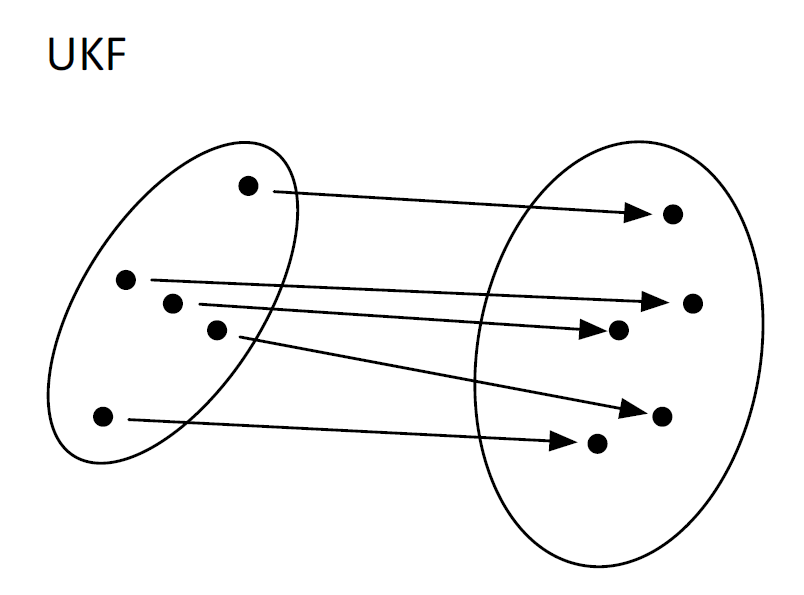
\includegraphics[width=.9\linewidth]{UKF_transform.PNG}
  \caption{UKF Transform}
  \label{fig:UKF_transform}
\end{subfigure}
\caption{Transforms from prior to posterior for (a) EKF \cite{Xmisc} and (b) UKF \cite{Xmisc}. The EKF handles nonlinearities by linearizing at a single point. The UKF instead computes values of the nonlinear function at many sigma points and fits a Gaussian to the resulting points.}
\label{fig:EKF_vs_UKF_transform}
\end{figure}
%\FloatBarrier


\subsubsection{Unscented transform}
Here we assume an $n$-dimensional Gaussian $\mathcal{N}(\mu,\Sigma)$. Instead of linearizing about the mean, the unscented transform propagates ``sigma points''---samples chosen to represent the probability distribution---through the nonlinear function $g$. There are a total of $2n+1$ sigma points (numbered $i = 0, \dots, 2n$): one point at the mean and two points symmetrically  distributed according to the covariance in each of the $n$ dimensions.
\begin{align}
\begin{split}
\mathcal{X}^{[0]} &= \mu \\
\mathcal{X}^{[i]} &= \mu + \left(\sqrt{(n+ \lambda)\Sigma}\right)_i \qquad \text{for $i = 1, \dots, n$} \\
\mathcal{X}^{[i]} &= \mu - \left(\sqrt{(n+ \lambda)\Sigma}\right)_{i-n} \qquad \text{for $i = n+1, \dots, 2n$},
\end{split}
\label{UKFsigpts}
\end{align}
where $\lambda = \alpha^2(n+\kappa) - n$, and $\alpha$ and $\kappa$ parameterize the distance from the off-mean sigma points $\mathcal{X}^{[i]}$ from the mean $\mathcal{X}^{[0]}$. In calculating the sigma points (for instance in Algorithm \ref{UKF_ALG}), we use the notation $\gamma = \sqrt{n + \lambda}$.
Each sigma point is associated with two weights: $w_m^{[i]}$, used to compute the mean, and $w_c^{[i]}$, used to compute the covariance.
\begin{align}
\begin{split}
w_m^{[0]} &= \frac{\lambda}{n + \lambda}, \qquad w_c^{[0]} = \frac{\lambda}{n + \lambda} + (1 - \alpha^2 + \beta) \\
w_m^{[i]} &= w_c^{[i]} = \frac{1}{2(n+\lambda)} \qquad \text{for $i = 1, \dots, 2n$}.
\end{split}
\label{UKFweights}
\end{align}
A value of $\beta = 2$ is typically used \cite{thrun2005probabilistic}.
After computing the sigma points, we pass them through the nonlinear dynamics function,
\begin{equation}
	 \mathcal{Y}^{[i]} = g( \mathcal{X}^{[i]})
\end{equation}
Then given the weights we have chosen, we are able to recover the mean and covariance of the distribution,
\begin{align}
\begin{split}
\mu' &= \sum_{i=0}^{2n} w_m^{[i]}\mathcal{Y}^{[i]}\\
\Sigma' &= \sum_{i=0}^{2n} w_c^{[i]}(\mathcal{Y}^{[i]}-\mu')(\mathcal{Y}^{[i]}-\mu')^{T}
\end{split}
\end{align}

\subsubsection{UKF Algorithm}
The UKF algorithm takes the same inputs as the other variants of the Kalman filter: the probability distribution of the state at the previous timestep, as well as the current control input and measurement. At each time step, we compute the sigma points and then propagate them through the dynamics equation:
\begin{equation}
\bar{\mathcal{X}}^*_t = g(u_t, \mathcal{X}_{t-1})
\end{equation}
Note that $\bar{\mathcal{X}}^*_t$ do not necessarily correspond to a Gaussian distribution (i.e., maintain their symmetry) after this nonlinear transformation. Then, from $\bar{\mathcal{X}}^*_t$, we can compute the \textit{predicted belief} $(\bar{\mu}_t, \bar{\Sigma}_t)$ using the weighting as shown in \eqref{UKFweights}:
\begin{align}
\begin{split}
\bar{\mu}_t &= \sum_{i=0}^{2n} w_m^{[i]}\bar{\mathcal{X}_t^*}^{[i]} \\
\bar{\Sigma}_t &= \sum_{i=0}^{2n} w_c^{[i]}\left(\bar{\mathcal{X}_t^*}^{[i]} -\bar{\mu}_t\right)\left(\bar{\mathcal{X}_t^*}^{[i]} -\bar{\mu}_t\right)^T + R_t
\end{split}
\end{align}
We compute the predicted sigma-points $\bar{\mathcal{X}}_t$ from the predicted belief $(\bar{\mu}_t, \bar{\Sigma}_t)$ as follows, using the same rules as in \eqref{UKFsigpts}.
Propagating the sigma points through the nonlinear measurement function gives
\begin{equation}
\bar{\mathcal{Z}}_t = h(\bar{\mathcal{X}}_t),
\end{equation}
from which the predicted observation can be computed:
\begin{align}
\begin{split}
\hat{z}_t &=  \sum_{i=0}^{2n} w_m^{[i]}\bar{\mathcal{Z}_t}^{[i]} \\
S_t &= \sum_{i=0}^{2n} w_c^{[i]}\left(\bar{\mathcal{Z}_t}^{[i]} -\hat{z}_t\right)\left(\bar{\mathcal{Z}_t}^{[i]} -\hat{z}_t\right)^T + Q_t
\\\bar{\Sigma}_t^{x,z} &= \sum_{i=0}^{2n} w_c^{[i]}\left(\bar{\mathcal{X}_t}^{[i]} -\bar{\mu}_t\right)\left(\bar{\mathcal{Z}_t}^{[i]} -\hat{z}_t\right)^T
\end{split}
\end{align}
The quantity $S_t$ represents the uncertainty as the $(H_t \bar{\Sigma}_t H_t^T + Q_t)$ term in the EKF algorithm, while $\bar{\Sigma}_t^{x,z}$ describes the cross-covariance between the state and the measurement. Together, these two terms contribute to the Kalman gain:
\begin{equation}
K_t = \bar{\Sigma}_t^{x,z}S_t^{-1}
\end{equation}
Then we can update the belief function:
\begin{align}
\begin{split}
\mu_t &= \bar{\mu}_t + K_t(z_t - \hat{z}_t) \\
\Sigma_t &= \bar{\Sigma}_t  - K_t S_t K_t^T
\end{split}
\end{align}

\begin{algorithm}[H]
\caption{Unscented Kalman Filter}
\KwData{$(\mu_{t-1}, \Sigma_{t-1}), u_t, z_t$}
\KwResult{$\left(\mu_t, \Sigma_t\right)$}
$ \mathcal{X}_{t-1} = \left(\mu_{t-1} \qquad \mu_{t-1} + \gamma \sqrt{\Sigma_{t-1}}\qquad \mu_{t-1} - \gamma \sqrt{\Sigma_{t-1}}\right)$ \;
$\bar{\mathcal{X}}^*_t = g(u_t, \mathcal{X}_{t-1})$ \;
$\bar{\mu}_t = \sum_{i=0}^{2n} w_m^{[i]}\bar{\mathcal{X}_t^*}^{[i]}$ \;
$\bar{\Sigma}_t = \sum_{i=0}^{2n} w_c^{[i]}\left(\bar{\mathcal{X}_t^*}^{[i]} -\bar{\mu}_t\right)\left(\bar{\mathcal{X}_t^*}^{[i]} -\bar{\mu}_t\right)^T + R_t$ \;
$ \bar{\mathcal{X}}_{t} = \left(\bar{\mu}_{t} \qquad \bar{\mu}_{t}  + \gamma \sqrt{\bar{\Sigma}_t}\qquad \bar{\mu}_{t}  - \gamma \sqrt{\bar{\Sigma}_t}\right)$ \;
$\bar{\mathcal{Z}}_t = h(\bar{\mathcal{X}}_t)$\;
$\hat{z}_t =  \sum_{i=0}^{2n} w_m^{[i]}\bar{\mathcal{Z}_t}^{[i]}$ \;
$S_t = \sum_{i=0}^{2n} w_c^{[i]}\left(\bar{\mathcal{Z}_t}^{[i]} -\hat{z}_t\right)\left(\bar{\mathcal{Z}_t}^{[i]} -\hat{z}_t\right)^T + Q_t$ \;
$\bar{\Sigma}_t^{x,z} = \sum_{i=0}^{2n} w_c^{[i]}\left(\bar{\mathcal{X}_t}^{[i]} -\bar{\mu}_t\right)\left(\bar{\mathcal{Z}_t}^{[i]} -\hat{z}_t\right)^T$ \;
$K_t = \bar{\Sigma}_t^{x,z}S_t^{-1}$ \;
$ \mu_t = \bar{\mu}_t + K_t(z_t - \hat{z}_t)$ \;
$\Sigma_t = \bar{\Sigma}_t  - K_t S_t K_t^T$ \;
\KwReturn{$(\mu_t, \Sigma_t)$}
\label{UKF_ALG}
\end{algorithm}

\subsubsection{UKF Results}
%\FloatBarrier
\begin{figure}[t]
\centering
\begin{subfigure}{.5\textwidth}
  \centering
  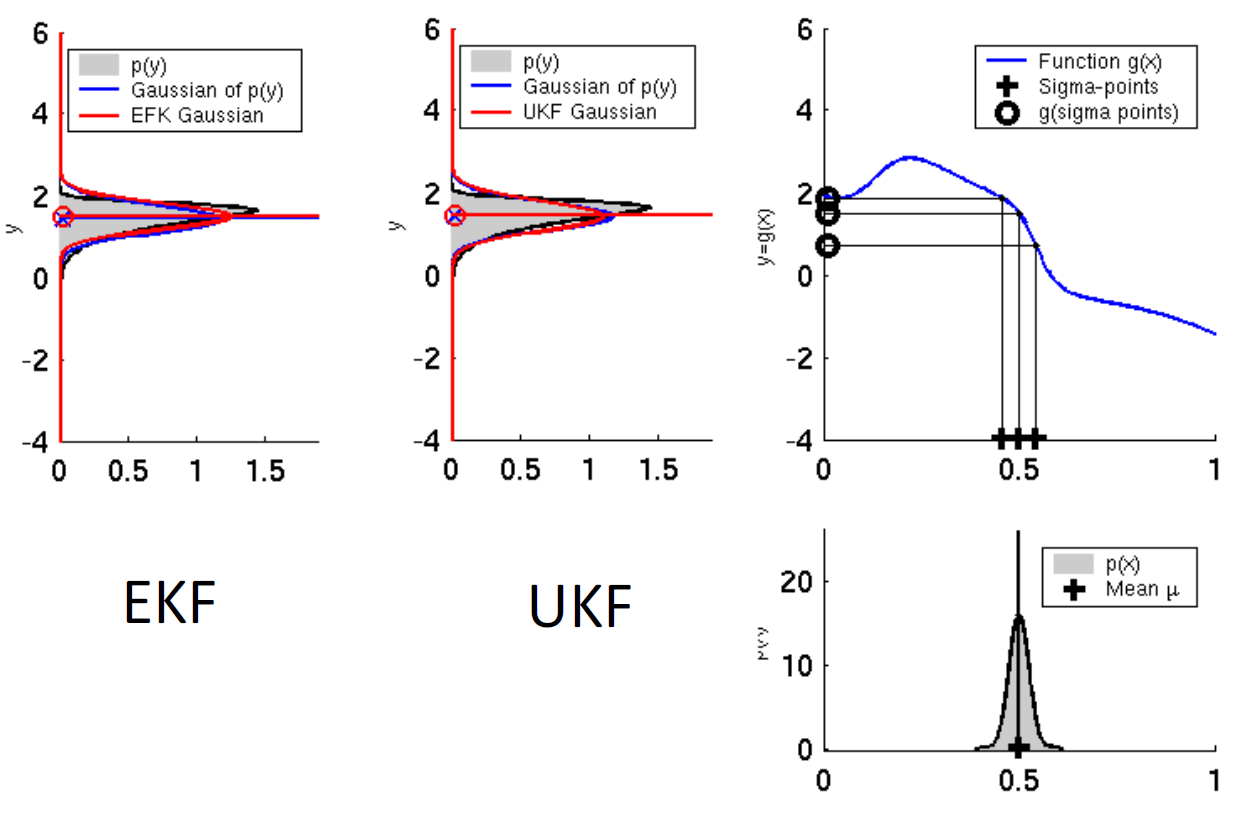
\includegraphics[width=.9\linewidth]{UKF_low_var.png}
  \caption{UKF with Low Variance}
  \label{fig:UKF_low}
\end{subfigure}%
\begin{subfigure}{.5\textwidth}
  \centering
  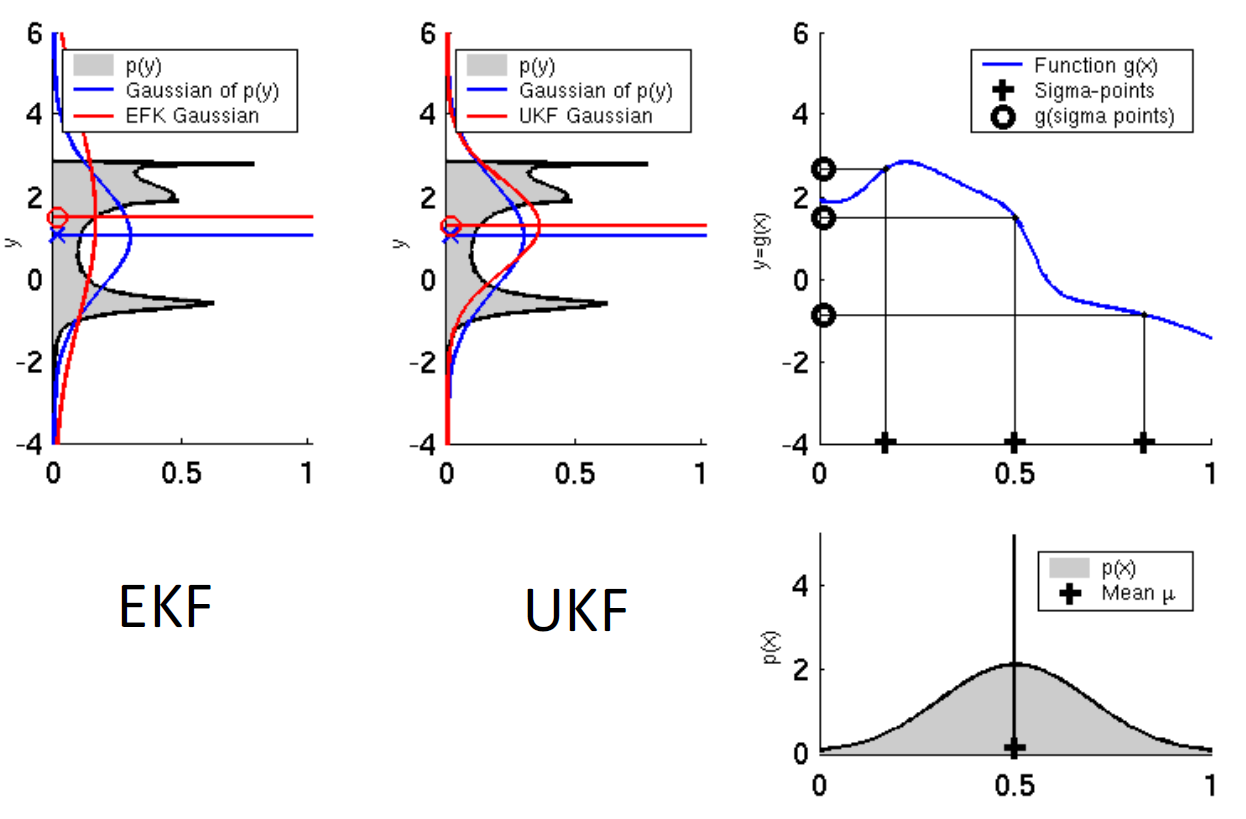
\includegraphics[width=.9\linewidth]{UKF_high_var.png}
  \caption{UKF with High Variance}
  \label{fig:UKF_high}
\end{subfigure}
\caption{The performance of the UKF compared to the EKF for different levels of uncertainty \cite{Xmisc}.}
\label{fig:UKF_variance}
\end{figure}
%\FloatBarrier
While the asymptotic complexities for the UKF and EKF algorithms are equivalent, the EKF is typically marginally faster than the UKF in practice. However, the UKF has the advantage if not requiring computation of Jacobians, which can sometimes pose an analytic challenge.
The UKF is much less sensitive to variance than the EKF because it propagates forward the exact nonlinear motion and measurement processes. As Figure \ref{fig:UKF_variance} shows, the UKF and EKF perform very similarly with low variance, but the UKF outperforms the EKF with high variance.


\section{Nonparametric Filters}
Nonparametric filters do not make any assumptions on the robot's belief distribution. Instead, they approximate the distribution discretely with a finite number of values. The accuracy of the representation depends on the number of values used, which results in a trade-off between expressiveness and computational burden. They are more robust to nonlinearities and discontinuities in the inference space, but also tend to be more complicated and time-consuming to implement.

\subsection{Histogram Filter}

Histogram filters are one way of finding a discrete approximation of a continuous distribution of beliefs. They first decompose a continuous space into finitely many bins,
\begin{equation}
\mathtt{dom}(X_t) = x_{1,t} \cup x_{2,t} \cup ... x_{k,t}
\end{equation}
then each region $x_{k,t}$ is assigned a probability $p_{k,t}$, which is approximated in a piecewise scheme based on the assumption of uniform density in each bin.
\begin{equation}
p(x_t) = \frac{p_{k,t}}{\lvert x_{k,t} \rvert},\quad x_t \in x_{k,t}
\end{equation}
To calculate the probability distribution, the motion and measurement models are discretized, and the central mass in each region is chosen as its representative state $\hat x_{k,t}$,
\begin{equation}
\hat x_{k,t} = \lvert x_{k,t} \rvert ^{-1}\int_{x_{k,t}}x_t d x_t
\end{equation}
Given a state $x_{k,t}$, the conditional probability $p(z_t \mid x_{k,t})$ is set equal to the probability of that measurement conditional on the representative state in that region, $p(z_t \mid \hat x_{k,t})$. A similar process is used to approximate the state transition probabilities by applying Bayes' law,
\begin{equation}
p(x_{k,t} \mid u_t, x_{i,t-1}) = \eta \lvert x_{k,t} \rvert p(\hat x_{k,t} \mid u_t, \hat x_{i,t-1})
\end{equation}
Finally, we execute a discrete Bayes' filter on the discretized probabilities to estimate the full belief distribution. A histogram representation of a robot's belief is shown in Figure \ref{fig:Histogram_belief}.


%\FloatBarrier
\begin{figure}[t]
\centering
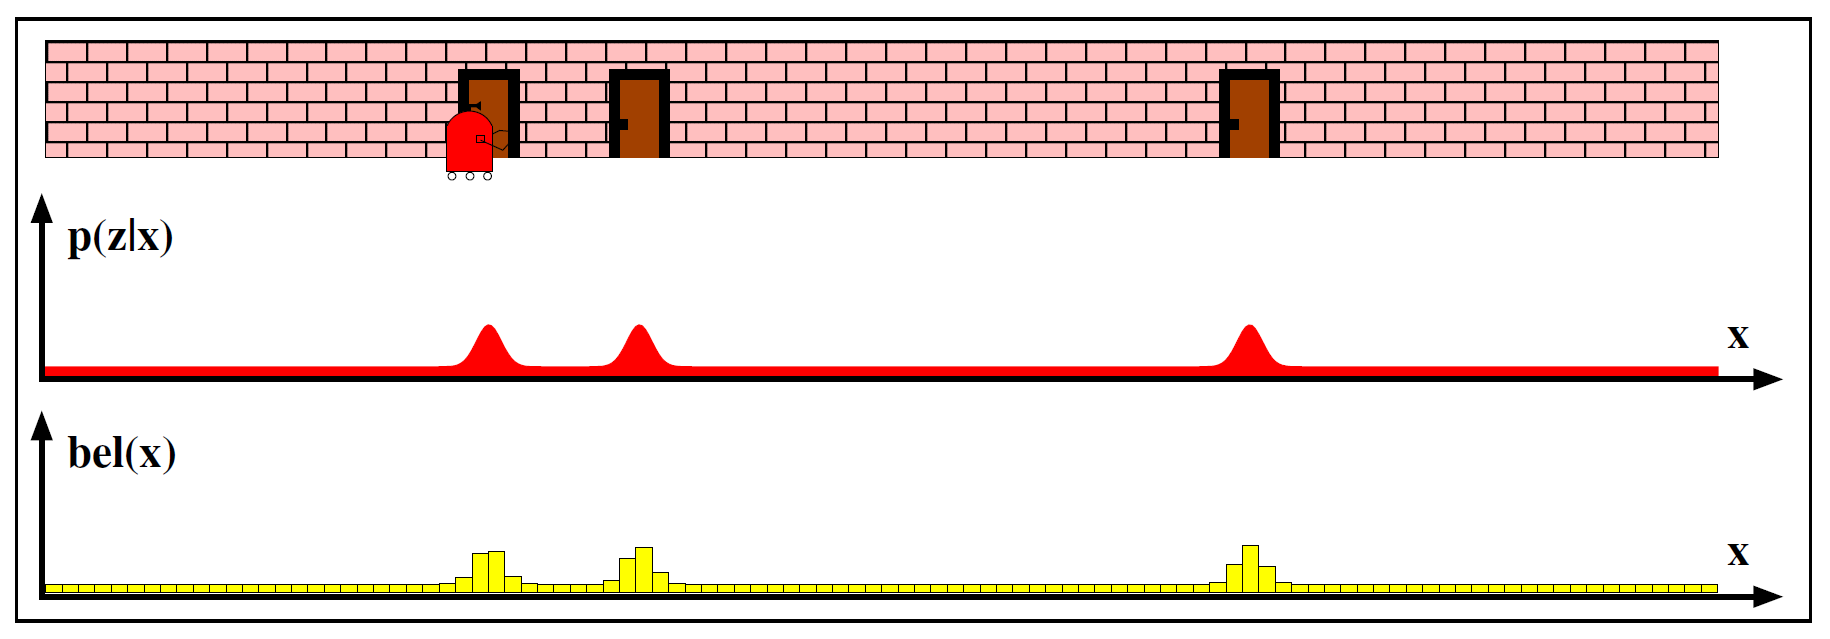
\includegraphics[width=1\linewidth]{histogram_belief.png}
\caption{Histogram representation of belief from initial sensor measurement from \cite{thrun2005probabilistic}.}
\label{fig:Histogram_belief}
\end{figure}
%\FloatBarrier


\subsection{Particle Filter}

A particle filter approximates the posterior distribution with a finite number of particles, denoted as
\begin{equation}
	\mathcal{X}_t = x_t^{[1]}, x_t^{[2]},..., x_t^{[M]}
\end{equation}
with each $x_t^{[k]}$ representing a hypothesis of what the true world state would be at time $t$. The denser the particles, the higher the probability of landing in a region. The algorithm operates iteratively: given $\mathcal{X}_{t-1}$, we construct the next particle set $\mathcal{X}_t$ by resampling $\mathcal{X}_{t-1}$ to correct the predicted belief function, incorporating our measurements into the calculation. This is done by computing the probability we observe a particular measurement conditional on the state, then drawing particles with replacement using these probabilities.

After resampling, particles are distributed as
\begin{equation}
	bel(X_t) = \eta P(z_t \mid x_t^{[m]})\overline{bel}(X_t)
\end{equation}
for $M \rightarrow \infty$. That is, in the limit, we recover the distribution of the true nonlinear filter. ($M \approx 1000$ achieves acceptable accuracy in practice). A few iterations of the particle filter algorithm for robot localization are shown in Figure \ref{fig:Particle_filter}.

\begin{algorithm}[H]
\caption{Particle Filter}
\KwData{$\mathcal{X}_{t-1}, u_t, z_t$}
\KwResult{$\mathcal{X}_t$}
$\bar{\mathcal{X}}_t = X_t = \emptyset$\;
\For{$m=1$ \KwTo $M$}{
sample $x_t^{[m]} \sim p(x_t \mid u_t, x_{t-1}^{[m]})$\;
$w_t^{[m]} = p(z_t \mid x_t^{[m]})$\;
$\bar{\mathcal{X}}_t = \bar{\mathcal{X}}_t \cup \left(x_t^{[m]}, w_t^{[m]}\right)$\;
}
\For{$i=1$ \KwTo $M$}{
draw $i$ with probability $\propto w_t^{[i]}$\;
add $x_t^{[i]}$ to $\mathcal{X}_t$\;
}
\KwReturn{$\mathcal{X}_t$}
\end{algorithm}

%\FloatBarrier
\begin{figure}[p]
\centering
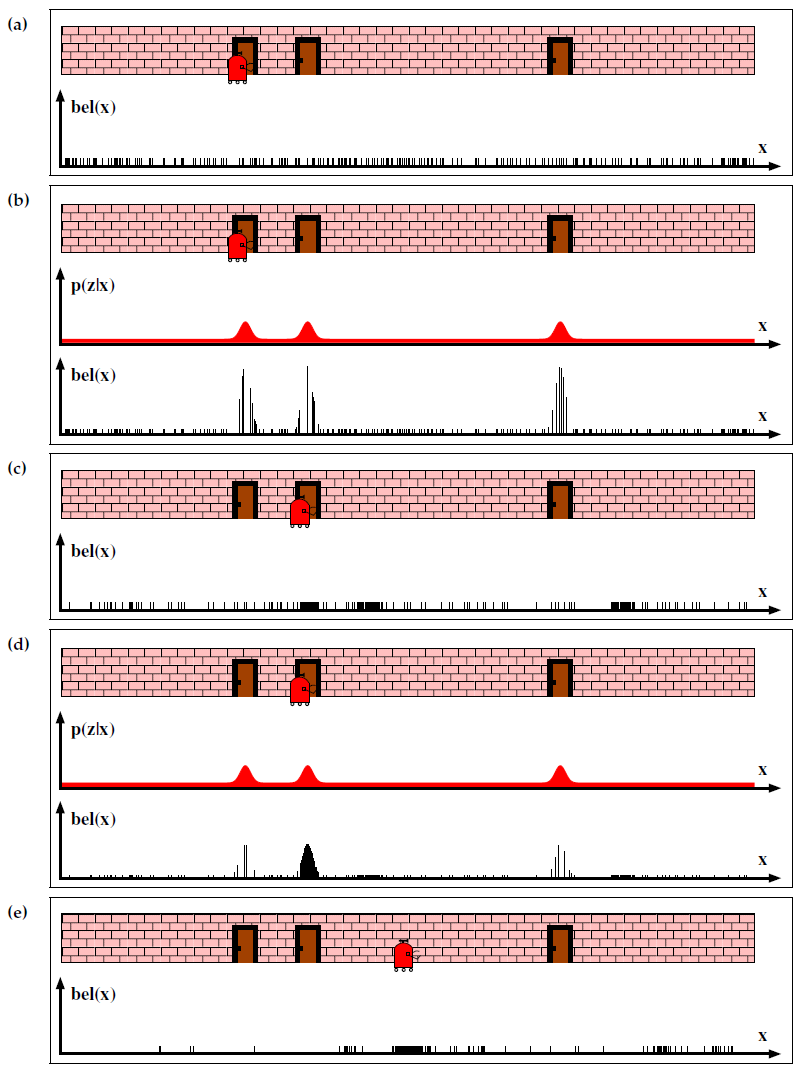
\includegraphics[width=0.88\linewidth]{particle_localization.png}
\caption{Particle filter used for robot localization from \cite{thrun2005probabilistic}: (a) Initial particles sampled uniformly over entire state space, (b) same set of particles from (a) after importance weighting with initial sensor measurement, (c) resampled particles from weighted distribution after motion, (d) importance weighting of new particle set with new sensor measurement, and (e) resampled particle set after further motion.}
\label{fig:Particle_filter}
\end{figure}
%\FloatBarrier

\section{Robot Localization}
Localization is the process of determining the correspondence between a robot's placement and the environment's map coordinates. Like before, a control input $u_t$ gives rise to a robot state $x_t$, which produces measurements $z_t$. The distinction is that this time, the map $m$ influences our measurements and possibly control parameters as well. Different situations thus may call for different filters. This influence is shown in the updated Bayes network (Hidden Markov Model) for robot localization in Figure \ref{fig:HMM_with_map}. Similarly, the influence of the map (door locations) can be seen in the measurement model $p(z \mid x)$ in Figures \ref{fig:Histogram_belief}, \ref{fig:Particle_filter}b, and \ref{fig:Particle_filter}d.

In position tracking, the initial pose of the robot is known with certainty. EKF works well for this problem because the belief distribution is concentrated (indeed, a point mass) at the mean. On the other hand, global localization assumes the initial pose is unknown, so nonparametric filters like histogram or particle filters are preferable. Finally, a case of theoretical interest arises if the initial pose is unknown and the robot can be "kidnapped" during its operation, i.e., a discontinuity may exist in its state $\mathbf{x}(t)$. This models the situation when a filter diverges to a significant enough degree that it must be reset. Hence, our localization algorithm should be capable of restarting from a different point/orientation in space. The kidnapped robot localization problem is best addressed with nonparametric, multi-hypothesis filters.

Environmental changes are another important consideration in mobile robot localization. A static environment assumes that the robot is the only object that moves. In contrast, a dynamic environmental model allows other objects, such as people, to move as well. This problem is usually addressed by augmenting the state vector or rejecting outliers.

Passive localization assumes that a single module takes measurements, and the robot's motion is unrelated to its localization process. A more sophisticated approach is active localization, where the robot's movement is aimed (at least partly) toward improving its understanding of the environment. For example, a robot in a corner will tend to reorient itself to face the rest of the room, so it can collect environmental information as it moves along the wall. In the same situation, a passively localized robot may simply slide along with its camera facing the wall.

Finally, a topic of current research is multi-robot localization: how can a team of robots cooperatively localize themselves within an environment?

%\FloatBarrier
\begin{figure}[H]
\centering
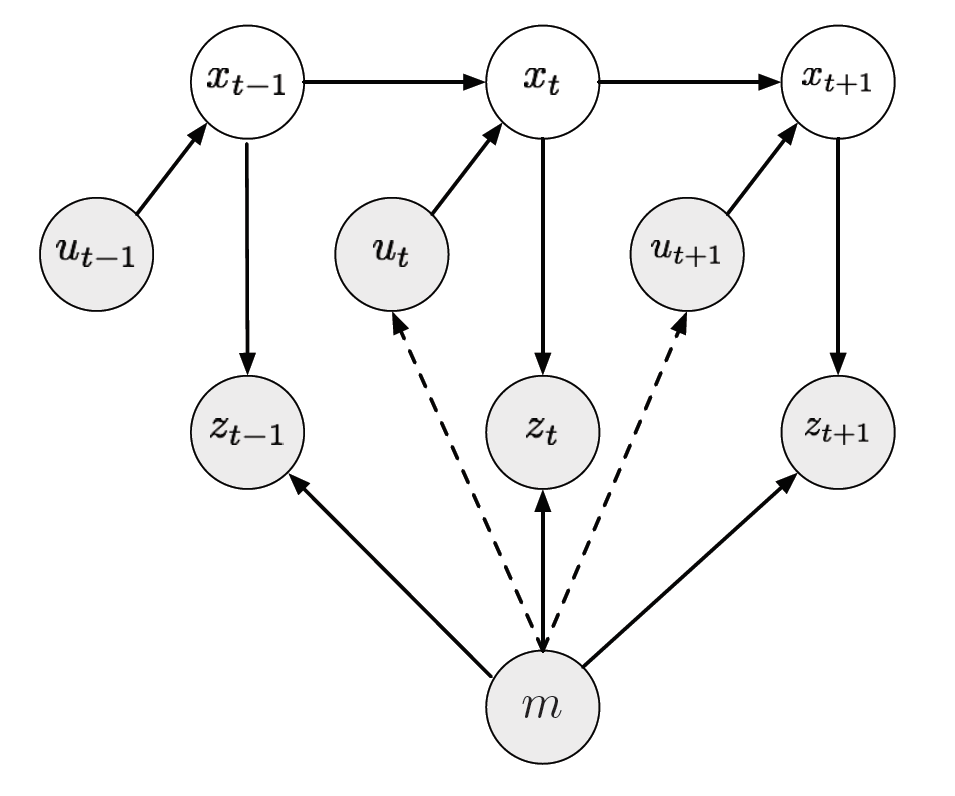
\includegraphics[width=0.45\linewidth]{HMM_w_map.png}
\caption{Hidden Markov Model for robot localization, where a map informs sensor measurements and control actions \cite{Xmisc}.}
\label{fig:HMM_with_map}
\end{figure}
%\FloatBarrier

\printbibliography

\end{document}